\documentclass[tikz,border=2mm]{standalone}
\definecolor{structure}{HTML}{1A535C}
\definecolor{main}{HTML}{C6892A}
\definecolor{second}{HTML}{2E4057}
\definecolor{third}{HTML}{8B2635}

\begin{document}

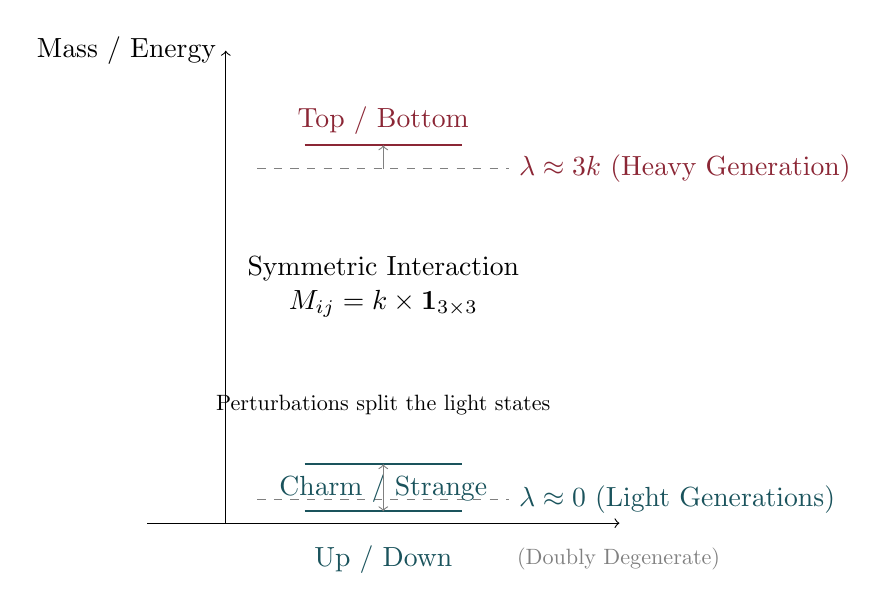
\begin{tikzpicture}[xscale=2, yscale=1.5]

% Plot Frame
\draw[->] (0,0) -- (0, 4) node[left] {Mass / Energy};
\draw[->] (-0.5,0) -- (2.5, 0);

% Unperturbed Levels (Geometric)
\draw[dashed, gray] (0.2, 3) -- (1.8, 3);
\node[right, color=third] at (1.8, 3) {$\lambda \approx 3k$ (Heavy Generation)};

\draw[dashed, gray] (0.2, 0.2) -- (1.8, 0.2);
\node[right, color=structure] at (1.8, 0.2) {$\lambda \approx 0$ (Light Generations)};
\node[right, gray, scale=0.8] at (1.8, -0.3) {(Doubly Degenerate)};

% Levels with splitting
\draw[thick, third] (0.5, 3.2) -- (1.5, 3.2) node[midway, above] {Top / Bottom};
\draw[->, gray] (1, 3) -- (1, 3.2);

\draw[thick, structure] (0.5, 0.5) -- (1.5, 0.5) node[midway, below] {Charm / Strange};
\draw[thick, structure] (0.5, 0.1) -- (1.5, 0.1) node[midway, below=3mm] {Up / Down};
\draw[->, gray] (1, 0.2) -- (1, 0.5);
\draw[->, gray] (1, 0.2) -- (1, 0.1);

% Annotations
\node[align=center] at (1, 2) {Symmetric Interaction \\ $M_{ij} = k \times \mathbf{1}_{3\times3}$};
\node[align=center, scale=0.8] at (1, 1) {Perturbations split the light states};

\end{tikzpicture}

\end{document}
